\documentclass{standalone}

\usepackage{tikz}
\usepackage{amsmath,amsfonts,amssymb}
\usetikzlibrary{positioning, backgrounds}
\begin{document}
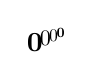
\begin{tikzpicture}
\clip (-0.09,-0.13) rectangle + (.47,.32);
\node [inner sep=0,outer sep=0,inner frame sep=0pt,tight background,draw=none] (first) at (0,0)  {$\mathbf{0}$};
\node [inner sep=0,outer sep=0,inner frame sep=0pt,tight background,draw=none,scale=.8] (second) at (0.135,0.05) {0};
\node [inner sep=0,outer sep=0,inner frame sep=0pt,tight background,draw=none,scale=.64] (third) at (0.24,0.09) {0};
\node [inner sep=0,outer sep=0,inner frame sep=0pt,tight background,draw=none,scale=.512] (fourth) at (0.33,0.125) {$\mathbf{0}$};  
\end{tikzpicture}
\end{document}\newcommand\thevector[4]{
\begin{tikzpicture}
    \draw (first){#1};
\end{tikzpicture}
}
\newcommand\A{\thevector{1}{0}{0}{0}}
\begin{document}
\A
\end{document}